%!TEX TS-program = xelatex
%!TEX encoding = UTF-8 Unicode

\documentclass[11pt,tikz,border=1]{standalone}
\usetikzlibrary{positioning}

\begin{document}
  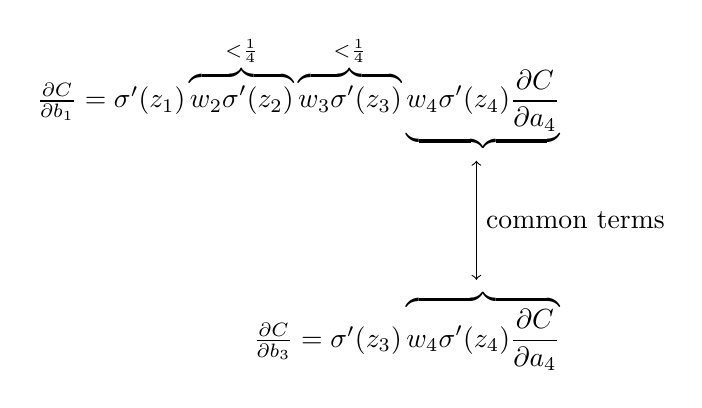
\begin{tikzpicture}

    \node (up) {
      $\frac{\partial C}{\partial b_1} = \sigma'(z_1) 
        \overbrace{w_2 \sigma'(z_2)}^{< \frac{1}{4}} 
        \overbrace{w_3 \sigma'(z_3)}^{< \frac{1}{4}} 
        \underbrace{w_4 \sigma'(z_4) \frac{\partial C}{\partial a_4}}$
    };
    
    \node (down) [below=3,anchor=east] at (up.east) {
      $\frac{\partial C}{\partial b_3} = \sigma'(z_3)
        \overbrace{w_4 \sigma'(z_4) \frac{\partial C}{\partial a_4}}$
    };
    
    \draw[<->] ([xshift=-1.185cm]up.south east) -- node [right] {common  terms} ([xshift=-1.185cm]down.north east);

  \end{tikzpicture} 
\end{document}
